\documentclass[14pt]{beamer}

%encoding
\usepackage[utf8]{inputenc}

%language
\usepackage[russian]{babel}
\usepackage{amsmath}
\usepackage{bm}
\usepackage{graphicx}
\usepackage{hyperref}
\usepackage{setspace}
\usepackage{tikz}
\usepackage{adjustbox}
\usepackage{marvosym}
\usepackage{animate}
\usetikzlibrary{shapes,arrows,positioning}
\makeatletter
\makeatother
\graphicspath{{images/}}

\usepackage{tikz}
\usetikzlibrary{shapes,arrows}

\tikzstyle{decision} = [diamond, draw, fill=blue!20, text width=4.5em, text badly centered, node distance=3cm, inner sep=0pt]
\tikzstyle{block} = [rectangle, draw, fill=blue!20, text width=11em, text centered, rounded corners, minimum height=2em]
\tikzstyle{line} = [draw, -latex    ]
\tikzstyle{cloud} = [draw, ellipse,fill=red!20, node distance=3cm, minimum height=2em]

\setbeamerfont{author in head/foot}{size=\small}
\setbeamerfont{title in head/foot}{size=\footnotesize}
\setbeamercovered{invisible}
\setbeamertemplate{navigation symbols}{}%remove navigation symbols

\title[Моделирование клапанов]{Математическое моделирование работы искусственного сердечного клапана}
\date{\today}
\author[Долгов Д.А.]{H. Miloshevich, Y.N. Zakharov, Y.I. Shokin, D.A. Dolgov, I.V. Grigorieva}
\institute{
    University of Pristina, Serbia\\
    Kemerovo State University, Kemerovo, Russia\\
    Institute of Computational Technologies of SB RAS, Novosibirsk, Russia\\
    \vspace{0.7cm}
}
\usetheme[numbers, totalnumbers, minimal, nologo]{Statmod}
\usefonttheme[onlymath]{serif}

\definecolor{statmodblue}{RGB}{100,10,30}
\definecolor{statmodsand}{RGB}{244,215,103}

\begin{document}
\maketitle

\begin{frame}
\frametitle{Содержание}
    \begin{itemize}
        \item[\MVRightarrow] Введение, актуальность и цели
        \item[\MVRightarrow] Математическая модель и метод решения
        \item[\MVRightarrow] Моделироввание сердечного клапана
        \item[\MVRightarrow] Моделирование аневризмы сосуда
    \end{itemize}
\end{frame}

%description of the problem
\begin{frame}
\frametitle{Введение}
Искусственные клапаны являются эффективным способом лечения многих
сердечно-сосудистых заболеваний. Их конструктивные особенности делают их одними
из самых сложных медицинских устройств, используемых в кардиохирургии.
Требования к функционированию клапанов очень велики - необходимо, чтобы он
минимизировал турбулентность, создавал небольшой объем регургитации, позволял
избегать зон застоя, разделения потока и т.д.
\end{frame}
\note{
    объем регургитации - объем обратного течения (из желудочка в атриум)

    Каждый год в мире
    проводится примерно 250 000 операций по восстановлению или замене
    поврежденных сердечных клапанов, и наблюдается тенденция к росту этого
    числа - Institute D.C.R. {\em Adult cardiac surgery database, executive summary} \url{http://www.sts.org/sites/default/files/documents/2015Harvest2_ExecutiveSummary.pdf}, 2015.

}

\begin{frame}
\frametitle{Обзор исследований}
    Существует множество исследований, которые расматривают только сам клапан и его деформации,
    представляя поток в упрощенном виде или получая данные о давлении экспериментально. См. например:\\
    \par
    {\tiny
        \begin{itemize}
            \item[\MVRightarrow] Бокерия Л.А., Скопин И.И., Сазоненков М.А., Тумаев Е.Н., Механическое напряжение в створках митрального клапана и биопротеза в митральной позиции. Влияние геометрии фиброзного кольца на величину напряжения створок/Клиническая физиология кровообращения, 2008, №2
            \item[\MVRightarrow] Сазоненков, М.А. Расчет напряжений в структурах нормального митрального клапана. / М.А. Сазоненков, Е.Н. Тумаев, И.И. Скопин // Бюллетень НЦ ССХ им. А.Н. Бакулева РАМН. Сердечно-сосудистые заболевания. Четырнадцатый Всероссийский съезд сердечно-сосудистых хирургов. – 2008. - Т 9, N 6. - с. 55.
            \item[\MVRightarrow] Kunzelman K.S., Reimink M.S. et al  Annular dilatation increases stress in the mitral valve and delays coaptation: a finite element computer model. (1997) Cardiovasc Surg 5(4):427–434
            \item[\MVRightarrow] Weinberg E. Dynamic simulation of heart mitral valve with transversely isotropic material model. Massachusetts Institute of Technology (2005)
            \item[\MVRightarrow] Kim H.S. Nonlinear multi-scale anisotropic material and structural models for prosthetic and native aortic heart valves. Georgia Institute of Technology (2009)
        \end{itemize}
    }
\end{frame}
\note{
    Отметить, что рассматриваются работы, посвященные именно математическому моделированию клапанов,
    а не экспериментальному. На эту тему мало русскоязычных работ - даже в монографии "Искусственные клапаны сердца"
    (Орловский, Гриценко, Юхнев, Евдокимов, Гавриленков),
    где описан крупный вклад отечественных ученых в области клапанов, в разделе "Математическое моделирование" нет
    упоминаний о русскоязычных работах.
    Существует достаточно много (по крайней мере, зарубежных) исследований,
    посвященных математическому моделированию сердечных клапанов. В ранних моделируются
    только достаточно простые клапаны (по структуре, двумерные и проч.).
    Существует много современных работ, которые изучают клапан только с точки зрения
    эластичности, напряжений, возникающих при деформации и проч (при этом данные о давлении жидкости
    берутся либо из эксперимента, либо упрощенные, например течение Пуазеля).
    Самый перспективный вид исследований те, которые полноценно описывают взаимодействие потока и клапана,
    т.е. IBM
}

\begin{frame}
\frametitle{Обзор исследований}
    Исследования, которые рассматривают полноценное взаимодействие ''жидкость-клапан'', зачастую относятся
    к методу погруженной границы, т.к. он позволяет считать клапан сколь угодно тонким. Практически нет
    известных нам русскоязычных работ по этой теме, а в существующих англоязычных мало освещена тема потока
    жидкости с примесями:
    \par
    {\tiny
        \begin{itemize}
            \item[\MVRightarrow] Орловский П.И., Гриценко В.В., Юхнев А.Д., Евдокимов С.В., Гавриленков В.И. Искусственные клапаны сердца. СПб. 2007. - 448с
            \item[\MVRightarrow] Peskin, Charles S. "Numerical analysis of blood flow in the heart." Journal of computational physics 25.3 (1977): 220-252.
            \item[\MVRightarrow] Luo, X. Y., et al. "Effect of bending rigidity in a dynamic model of a polyurethane prosthetic mitral valve." Biomechanics and modeling in mechanobiology 11.6 (2012): 815-827.
            \item[\MVRightarrow] Flamini, Vittoria, Abe DeAnda, and Boyce E. Griffith. "Immersed boundary-finite element model of fluid-structure interaction in the aortic root." (2015).
        \end{itemize}
    }
\end{frame}

\begin{frame}
\frametitle{Цели}
    \begin{itemize}
        \item[\MVRightarrow] Разработка технологии решения нестационарной трехмерной задачи о движении створок искусственного клапана внутри крупных кровеносных сосудов и деформации их стенок под давлением потока жидкости с учетом неоднородной структуры крови.
        \item[\MVRightarrow] Моделирование работы клапана <<Юнилайн>> и верификация результатов с помощью экспериментальных данных
    \end{itemize}
\end{frame}
\note{
    Для того, чтобы добиться этих целей, необходимо решить следующие задачи:

    *
}

\begin{frame}
\frametitle{Математическая модель и метод решения}
    \begin{itemize}
        \item[\MVRightarrow] Биологические характеристики системы
        \item[\MVRightarrow] Моделирование потока неоднородной жидкости
        \item[\MVRightarrow] Моделирование деформации створок клапана
        \item[\MVRightarrow] Взаимодействие <<жидкость-граница>>
    \end{itemize}
\end{frame}

% valves placement
\begin{frame}
\frametitle{Схема расположения клапанов}
    \begin{center}
        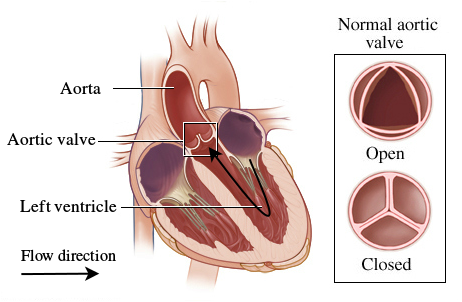
\includegraphics[width=8.5cm]{aorta_scheme.png}
    \end{center}
\end{frame}

\begin{frame}
\frametitle{Искусственный клапан}
    \begin{center}
        \vspace{1.0cm}
        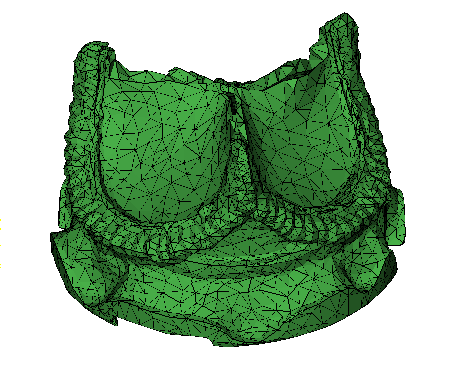
\includegraphics[width=6cm]{real_valve_3_1.png}
        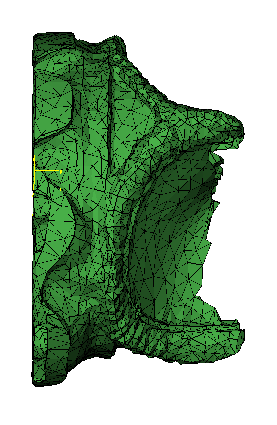
\includegraphics[width=3cm]{real_valve2_1.png}

        \vspace{1.1cm}
        \mbox{\scriptsize
            <<Юнилайн>>, ФГБУ НИИ КПССЗ СО РАМН, г. Кемерово
        }
    \end{center}
\end{frame}

% valve tissue structure
\begin{frame}
\frametitle{Схема строения тканей}
    \begin{center}
        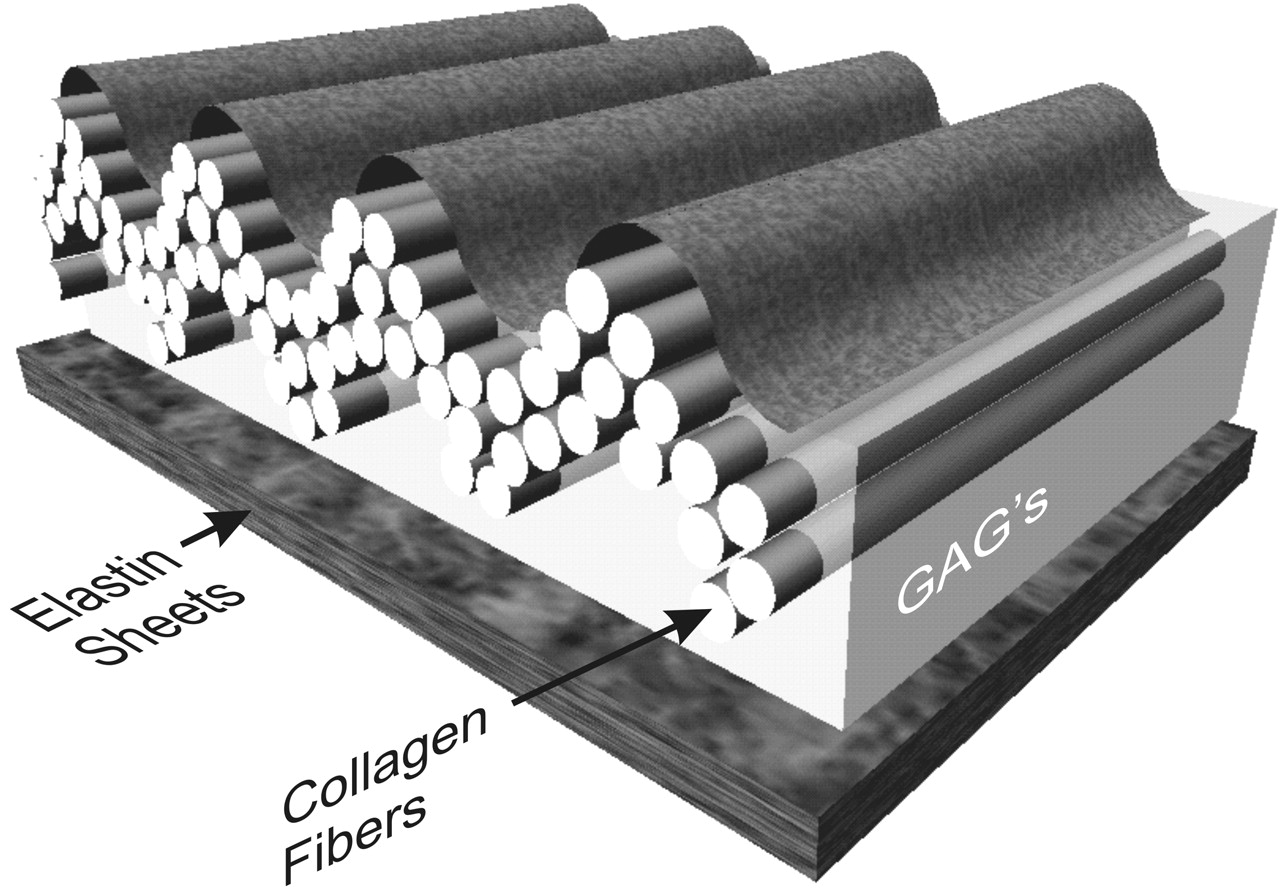
\includegraphics[width=8.5cm]{valve_tissue_structure.jpg}
    \end{center}

    \begin{spacing}{0.5}
        \mbox{\scriptsize
            Vesely, Ivan. <<Heart valve tissue engineering.>> Circulation research 97.8 (2005): 743-755.
        }
    \end{spacing}

\end{frame}
\note{
    \begin{itemize}
        \item коллагеновые волокна (collagen fibers)
        \item слой эластина (белок) (elastin sheet)
        \item гликозаминогликаны (glycosaminoglycan matrix)
    \end{itemize}
}

% blood structure scheme
\begin{frame}
\frametitle{Схема структуры крови}
    \begin{center}
        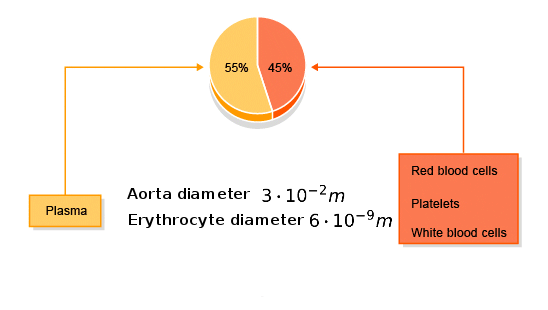
\includegraphics[width=8.5cm]{blood_scheme3.png}
    \end{center}
\end{frame}

\begin{frame}
\frametitle{Описание модели}
Рассмотрим задачу о течении крови внутри крупных сосудов с гибкими стенками и клапаном. Кровь является неоднородной и состоит из плазмы и взвешенных в ней форменных элементов. Клапан и стенки сосуда являются гибкими и изменяют свою форму под воздействием течения. Будем моделировать кровь как вязкую, несжимаемую двухкомпонентную жидкость, а стенки сосуда - как поверхность заданной формы, обладающую определенной жесткостью.
\end{frame}

%description of the problem: schema
\begin{frame}
\frametitle{Описание модели}
    \begin{center}
        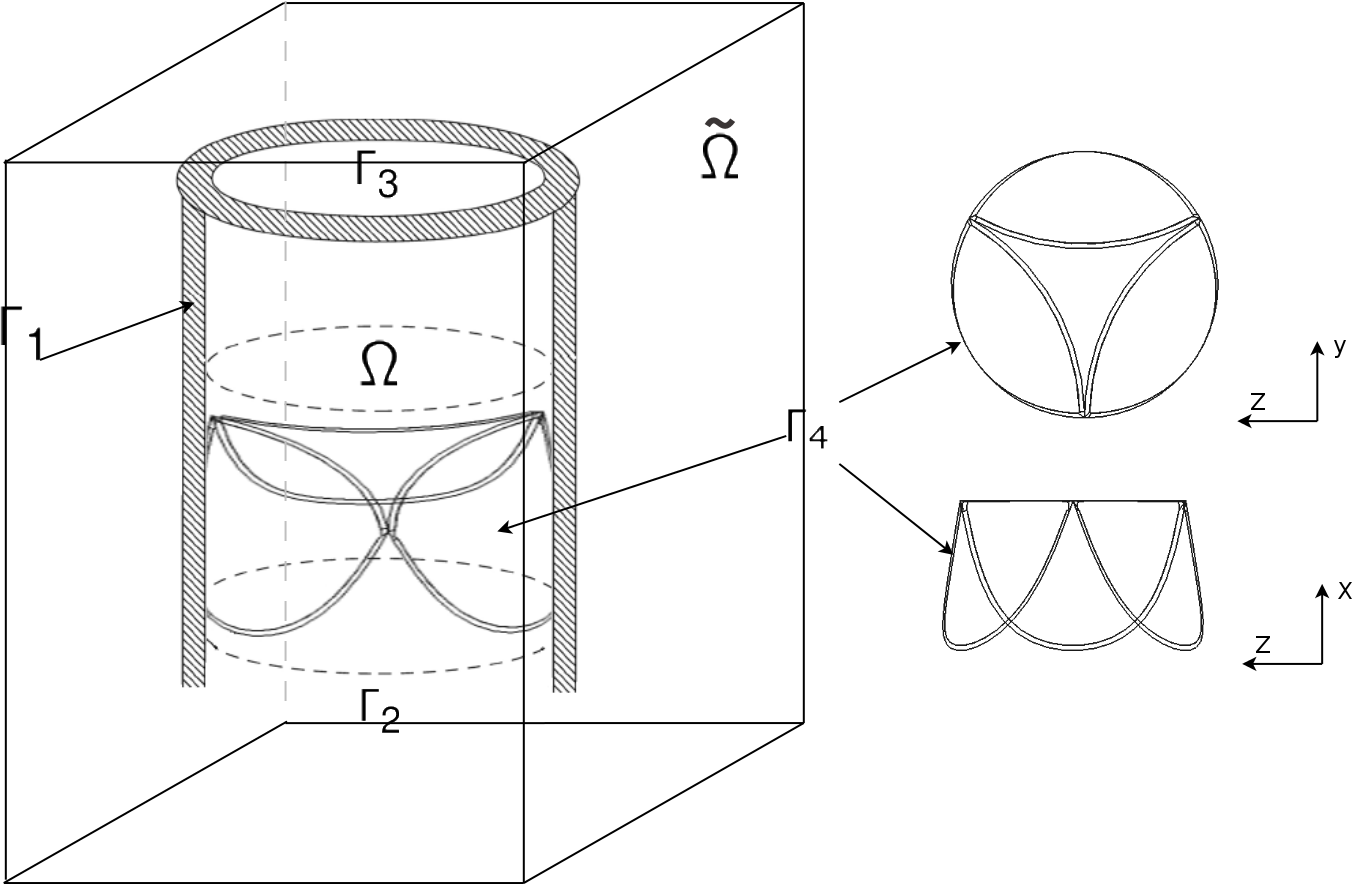
\includegraphics[width=10cm]{aorta_valve_scheme_flat_computation.png}
    \end{center}
\end{frame}
\note{$\Gamma_1$ - гибкие стенки, $\Gamma_2,\Gamma_3$ - вход/выход}

% navier stokes equations
\begin{frame}
\frametitle{Моделирование течения}
Система уравнений Навье-Стокса:
\begin{gather}
    \label{eq:motion}
    \frac{\partial u}{\partial t} + (u \cdot \nabla) u = - \frac{1}{\rho} \nabla p + \nabla \cdot \sigma + f\\
    \label{eq:continuity}
    \frac{\partial \rho}{\partial t} + \nabla \cdot (\rho u) = 0
\end{gather}
где $\sigma = \mu (\nabla u + (\nabla u)^{T})$, $\bar{x} = (x, y, z) \in \Omega$ с начальными и краевыми условиями
\begin{gather*}
    u(\bar{x}, t_0) = u_0;\ \frac{\partial u}{\partial n}|_{\Gamma_2, \Gamma_3} = 0\\
    p|_{\Gamma_2} = p_{in};\ p|_{\Gamma_3} = p_{out} \\
\end{gather*}

\end{frame}
\note{Уравнения записаны в векторном виде, $\sigma$ - вязкий тензор напряжений}

% concentration
\begin{frame}
\frametitle{Концентрация}
Уравнение для расчета концентрации примеси в жидкости:
\begin{gather}
    \label{eq:concentration}
    \frac{\partial c}{\partial t} + u \cdot \nabla c = 0
\end{gather}
с начальными и краевыми условиями
\begin{gather*}
    c(\bar{x}, 0) = c_0(\bar{x})\\
    c(\bar{x}, t)|_{\Gamma_2} = c_s(\bar{x}, t)
\end{gather*}

\end{frame}

% concentration: dependencies
\begin{frame}
\frametitle{Концентрация}
Плотность и вязкость зависят от концентрации:
\begin{gather}
    \label{eq:concentration_viscosity}
    \mu = c (\mu_2 - \mu_1) + \mu_1\\
    \label{eq:concentration_density}
    \rho = c (\rho_2 - \rho_1) + \rho_1
\end{gather}

где $\mu_1, \mu_2, \rho_1, \rho_2$ - вязкости и плотности обоих компонент.
\end{frame}

% boundary
\begin{frame}
\frametitle{Сопротивление деформации}
В каждой точке сосуда и клапана определена поверхностная сила, которая стремится вернуть систему в равновесное положение
\begin{gather}
    \label{eq:strain_energy}
    F =  \frac{\partial}{\partial s}(T \tau) + \frac{\partial^2}{\partial s^2} \Big( E \cdot I \frac{\partial^2}{\partial s^2} X \Big)
\end{gather}
\begin{gather}
    \label{eq:define_boundary_force}
    F = k \cdot \|X - X_0\|
\end{gather}
\end{frame}
\note{$E$ - модуль Юнга, $I$ - момент инерции поперечного сечения, $T$ - напряжение фибры, $\tau$ - единичный тангенциальный вектор, касательный к фибре.}

% solve method:immersed boundary
\begin{frame}
\frametitle{Взаимодействие}
Уравнения, описывающие взаимодействие погруженной границы и жидкости:
\begin{gather}
    \label{eq:ibm_velocity}
    \frac{\partial X}{\partial t} = \int_{\Omega_h} u \cdot \delta (\bar{x} - X)\; dx\; dy\; dz \\
    \label{eq:ibm_force}
    f = \int_{\Gamma_h} F \cdot \delta (\bar{x} - X)\; dq\; dr\; ds\\
    \label{eq:no_slip}
    \frac{\partial X}{\partial t} (q, r, s, t) = u(X(q, r, s, t), t)
\end{gather}
\end{frame}
\note{Заглавные символы относятся к погруженной границе, обычные - к жидкости}

% solve method
\begin{frame}
\frametitle{Метод решения}
Будем рассматривать отдельно задачи вычисления параметров течения жидкости и параметров движения стенок сосуда и клапанов. Для этого введем в расчетной области сетки:
\begin{itemize}
    \item[\MVRightarrow] $\Omega_h = \Omega_h(x, y, z)$ - равномерная разнесенная сетка для расчета течения
    \item[\MVRightarrow] $\Gamma_h = \Gamma_h(q, r, s, t)$ - дополнительная сетка, соотнесенная со стенками сосуда и лепестками клапана (в лагранжевых координатах)
\end{itemize}

\end{frame}
\note{При обтекании жидкость какого-либо тела, она испытвает влияние силы давления рядом с границей тела (и сдвиговые силы, если есть условие прилипания). Исходя их этого обтекание тела можно моделировать с помощью поля внешних сил}

% solve method:split scheme
\begin{frame}
\frametitle{Алгоритм решения: поток}
Схема расщепления по физическим факторам:
\begin{gather}
    \label{eq:split_first}
    \frac{u^* - u^n}{\triangle t} = - (u^n \cdot \nabla) u^n + \frac{1}{\rho} \nabla \sigma + f\\
    \label{eq:split_second}
    \rho \triangle p^{n+1} - (\nabla p \cdot \nabla p^{n+1}) = \frac{\rho^2 \nabla u^*}{\triangle t}\\
    \label{eq:split_third}
    \frac{u^{n+1} - u^*}{\triangle t} = - \frac{1}{\rho} \nabla p^{n+1}
\end{gather}
где $\nabla \sigma (u^n, \mu) = \mu \triangle u^n + (\nabla \mu \cdot \nabla) u^n + (\nabla \mu \cdot J_{u^n}) $
\end{frame}
\note{
    \begin{itemize}
        \item[\MVRightarrow] Решаем уравнение \eqref{eq:split_first} методом стабилизирующей поправки (Дугласа-Рекфорда)
        \item[\MVRightarrow] Из уравнения \eqref{eq:split_second} методом бисопряженных градиентов определяем поле давления
        \item[\MVRightarrow] Восстанавливаем окончательное поле вектора скорости по явным формулам \eqref{eq:split_third}
    \end{itemize}
}

% solve method: boundary forces
\begin{frame}
\frametitle{Алгоритм решения: клапан}
\begin{gather}
    \label{eq:strain_energy}
    F_{n} =  \frac{\partial}{\partial s}(T_{n} \tau_{n}) + \frac{\partial^2}{\partial s^2} \Big( E \cdot I \frac{\partial^2}{\partial s^2} X_{n} \Big)
\end{gather}
\end{frame}
\note{$E$ - модуль Юнга, $I$ - момент инерции поперечного сечения, $T$ - напряжение фибры, $\tau$ - единичный тангенциальный вектор, касательный к фибре.}

% solve method:ibm scheme
\begin{frame}
\frametitle{Взаимодействие}
Интерполяция скорости на погруженную границу и распределение силы сопротивления деформации:
\begin{gather}
    \label{eq:interpolation}
    U_n = \sum_{ijk}u_{ijk} \cdot D(x_{ijk} - x_n) h_{ijk}^3 \\
    \label{eq:spreading}
    f_{ijk} = \sum_n F_n \cdot D(x_{ijk} - x_n) h^2_n
\end{gather}

$D(x_n)$ соответствует $\delta(x - x_k)$.
\end{frame}

\begin{frame}
\frametitle{Моделирование сердечного клапана}
    \begin{itemize}
        \item[\MVRightarrow] Динамика идеального клапана
        \item[\MVRightarrow] Распределение примеси
        \item[\MVRightarrow] Эффект скручивания створок
        \item[\MVRightarrow] Динамика искусственного клапана <<Юнилайн>>
        \item[\MVRightarrow] Распределение напряжений
        \item[\MVRightarrow] Расход жидкости
    \end{itemize}
\end{frame}

% totals and examples
% use avconv -i video.avi -vsync 1 -r 10 -an -y 'data_%d.png'
% to create series of png for animation

\begin{frame}
\frametitle{Динамика идеального клапана}
    \animategraphics[autoplay,loop,width=\textwidth]{20}{animation/valve_delaunay3/data_}{1}{134}
\end{frame}

\begin{frame}
\frametitle{Распределение примеси}
    \animategraphics[autoplay,loop,width=\textwidth]{20}{animation/valve_in_mixture/data_}{1}{201}
\end{frame}

\begin{frame}
\frametitle{Эффект скручивания створок}
    \animategraphics[autoplay,loop,width=\textwidth]{20}{animation/rotation/data_}{1}{135}
\end{frame}

\begin{frame}
\frametitle{Динамика <<Юнилайн>>}
    \animategraphics[autoplay,loop,width=\textwidth]{20}{animation/real_valve/data_}{1}{108}
\end{frame}

\begin{frame}
\frametitle{Динамика <<Юнилайн>>}
    \animategraphics[autoplay,loop,width=\textwidth]{20}{animation/uniline_tracks/data_}{1}{108}
\end{frame}

\begin{frame}
\frametitle{Распределение напряжений}
    \begin{center}
        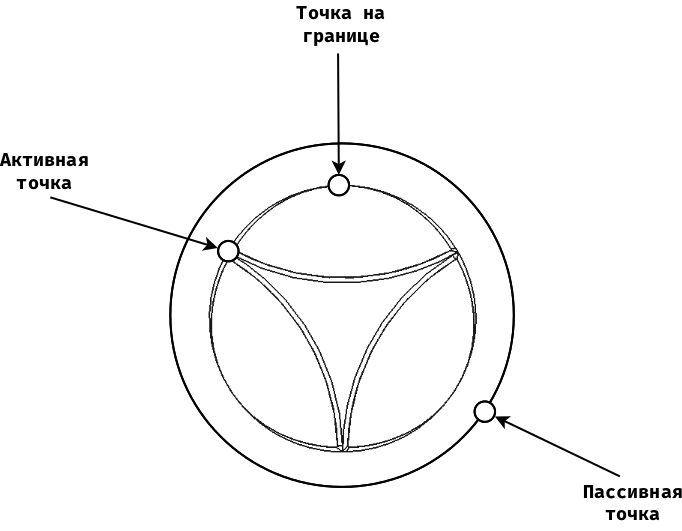
\includegraphics[width=9cm]{valve_points.png}
    \end{center}
\end{frame}

\begin{frame}
\frametitle{Распределение напряжений}
    \begin{center}
        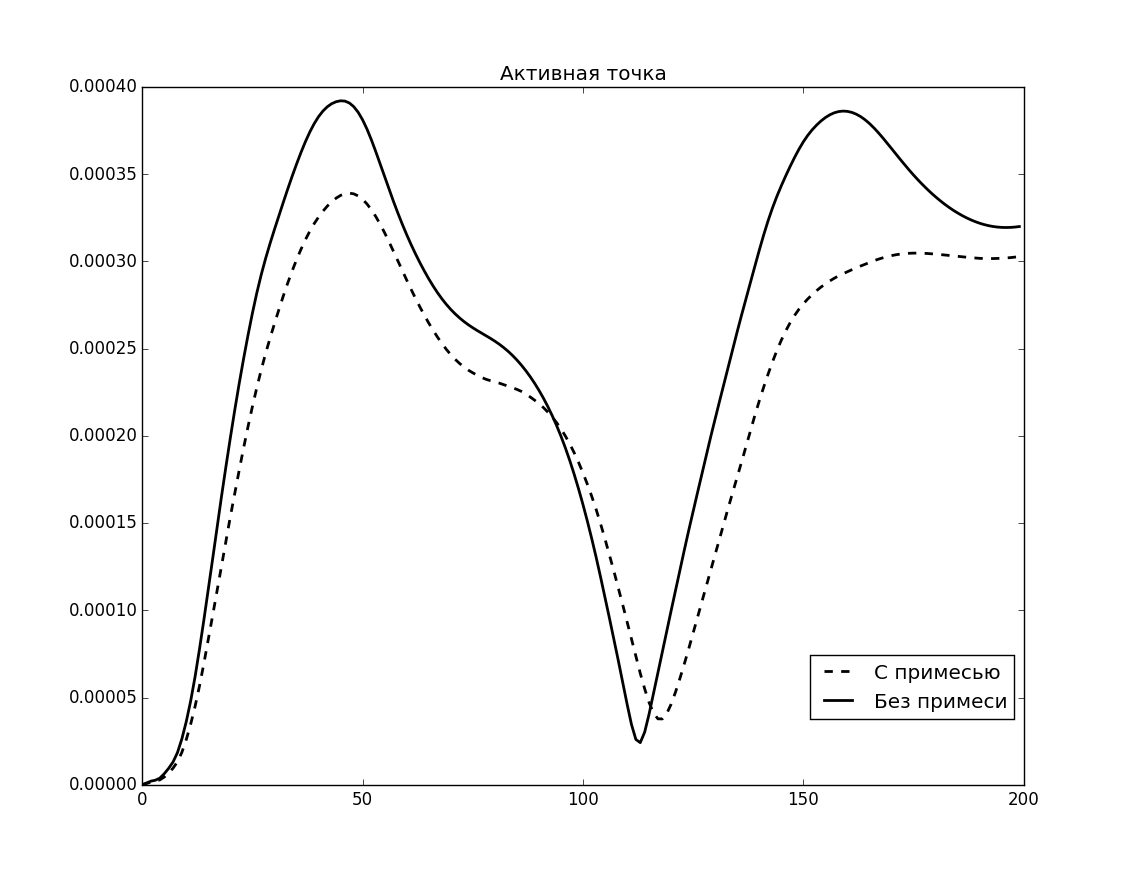
\includegraphics[width=10cm]{forces_active_point.png}
    \end{center}
\end{frame}

\begin{frame}
\frametitle{Распределение напряжений}
    \begin{center}
        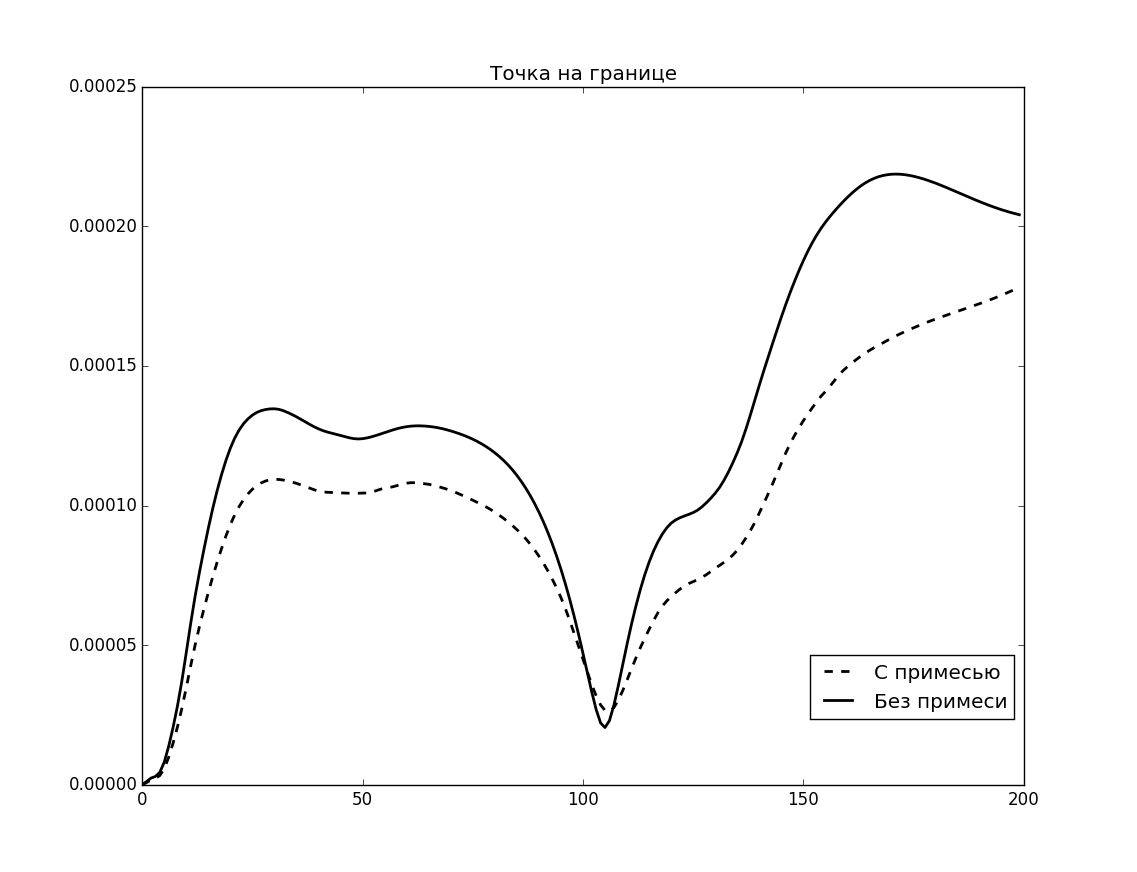
\includegraphics[width=10cm]{forces_boundary_point.png}
    \end{center}
\end{frame}

\begin{frame}
\frametitle{Распределение напряжений}
    \begin{center}
        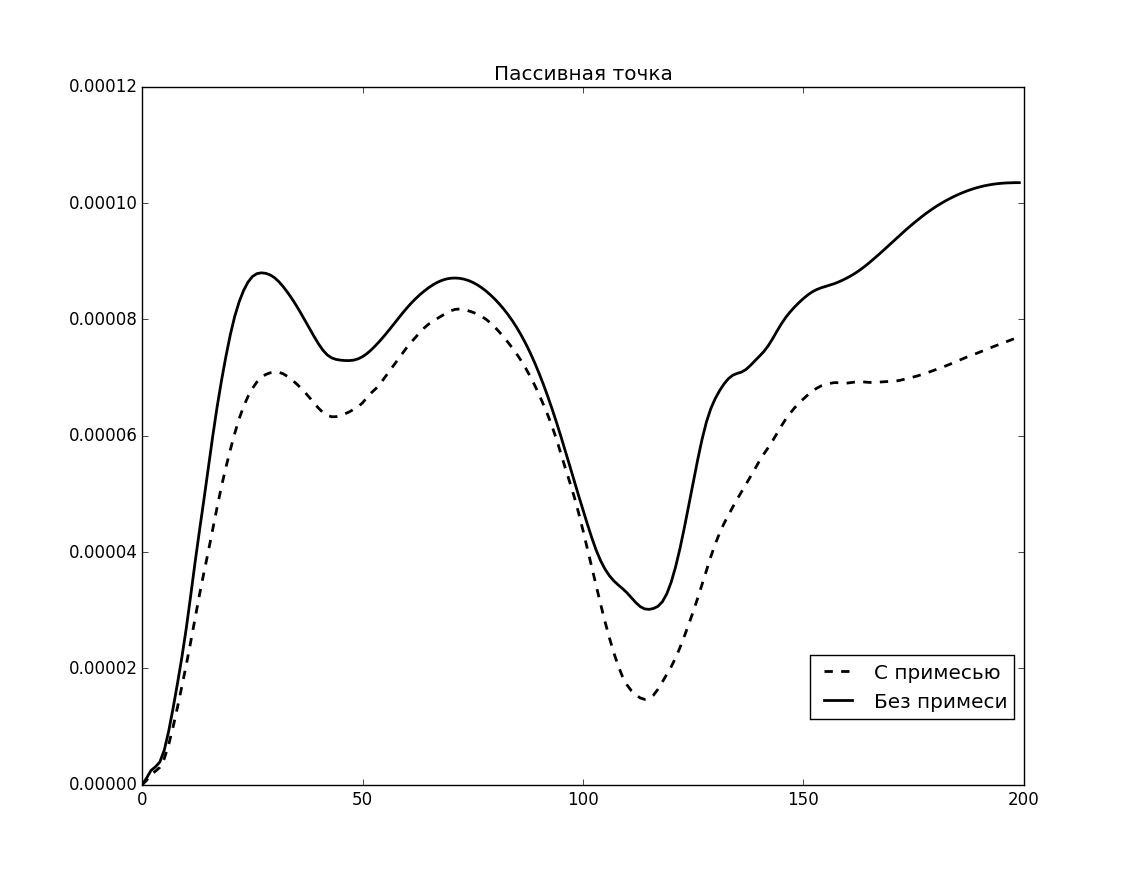
\includegraphics[width=10cm]{forces_passive_point.png}
    \end{center}
\end{frame}

\begin{frame}
\frametitle{Расход жидкости}
    \begin{center}
        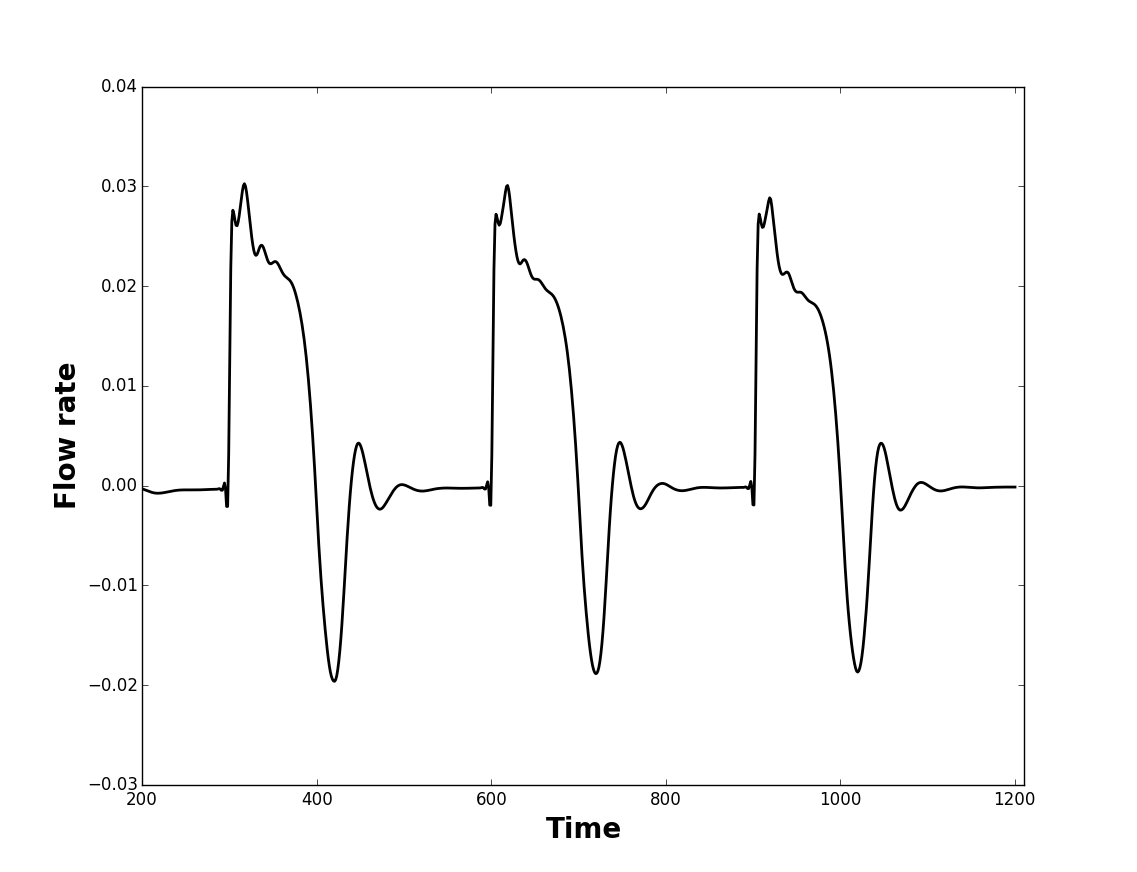
\includegraphics[width=10cm]{flowrate.png}
    \end{center}

    %\begin{adjustbox}{max totalsize={1.0\textwidth}{.7\textheight},center}
        %{\scriptsize
            %International Journal for Numerical Methods in Biomedical Engineering 28.3 (2012): 317-345.
            %%"Immersed boundary model of aortic heart valve dynamics with physiological driving and loading conditions." International Journal for Numerical Methods in Biomedical Engineering 28.3 (2012): 317-345.
        %}
    %\end{adjustbox}
\end{frame}

\begin{frame}
\frametitle{Моделирование аневризмы сосуда}
    \begin{itemize}
        \item[\MVRightarrow] Динамика движения жидкости и распределение скорости в сосуде с гибкими стенками разных форм
        \item[\MVRightarrow] Распространение примеси в сосуде с гибкими стенками разных форм
        \item[\MVRightarrow] Распространение примеси("тробма") при наличии стеноза небольшой степени
        \item[\MVRightarrow] Распространение примеси("тробма") при наличии стеноза большой степени
    \end{itemize}
\end{frame}

\begin{frame}
\frametitle{Динамика в сосуде с гибкими стенками}
    \animategraphics[autoplay,loop,width=10cm]{20}{animation/aneurysm_geom3/data_}{1}{98}
\end{frame}

\begin{frame}
\frametitle{Распределение скоростей}
    \animategraphics[autoplay,loop,width=10cm]{20}{animation/aneurysm_geom3_velocity/data_}{1}{98}
\end{frame}

\begin{frame}
\frametitle{Динамика в сосуде с гибкими стенками}
    \animategraphics[autoplay,loop,width=10cm]{20}{animation/aneurysm_geom1/data_}{1}{127}
\end{frame}

\begin{frame}
\frametitle{Распределение скоростей}
    \animategraphics[autoplay,loop,width=10cm]{20}{animation/aneurysm_geom1_velocity/data_}{1}{127}
\end{frame}

\begin{frame}
\frametitle{Распределение примеси}
    \animategraphics[autoplay,loop,width=10cm]{20}{animation/aneurysm_geom1_mixture/data_}{1}{103}
\end{frame}

\begin{frame}
\frametitle{Стеноз небольшой степени}
    \animategraphics[autoplay,loop,width=10cm]{20}{animation/thrombus_light_stenosis/data_}{1}{95}
\end{frame}

\begin{frame}
\frametitle{Стеноз большой степени}
    \animategraphics[autoplay,loop,width=10cm]{20}{animation/thrombus_strong_stenosis/data_}{1}{121}
\end{frame}

\begin{frame}
\frametitle{Заключение}
    \begin{itemize}
        \item[\MVRightarrow] Построенная модель работы искусственног сердечного
            клапана, учитывающая течения крови с переменной плотностью и
            вязкостью, а также гибкость створок клапана, позволяет получать физически непротиворечивые картины движения створок клапана и течения жидкости в сосудах с гибкими стенками для разных геометрий.
        \item[\MVRightarrow] Расчеты, проведенные для клапана <<Юнилайн>>,
            качественно согласуются с имеющимися данными, полученными
            экспериментально и из других исследований.
    \end{itemize}
\end{frame}

\end{document}
